\chapter{Background Theory}\label{chp:theory}

\section{Introduction}

\subsection{Chapter Scope}
This chapter contains the background theory which is necessary to understand the implementations in chapter \ref{chp:implementation} and how they are intended to work. Methods for vision based autonomous navigation is also discussed on a . 

\subsection{Brief Introduction to Computer Vision}
Computer Vision is the field of giving computers the ability to duplicate the way we perceive and understand our surroundings. This is not an easy task for several reasons. Much information is lost in the process of representing a 3d world on a 2d surface. As image processing really is digital signal processing in 2d, it is subject to irreversible information loss and noise through quantization. In short, the field of computer vision can be summed up to be the science of drawing conclusions about the real world based on pixel values in an image matrix, or a series of such matrices.

\subsection{Introduction to OpenCV}

\gls{opencv} is an  open source library with a vast number of advanced computer vision and machine learning algorithms. The library is written in C and C++; it supports Windows, Linux, iOS and Android; and has interfaces to Python, Java and MATLAB. All OpenCV applications in this project uses \gls{opencv} 3.0.0 for Windows. \gls{opencv} for Windows can be downloaded from \textit{sourceforge.net} or "itseez" on GitHub. The download from \textit{sourceforge.net} contains source files, sample programs, sample data and a pre-built library for MSVC 2010 and 2013. The pre-build library can quickly be plugged into  an IDE such as Qt Creator or Visual Studio 2013, thus giving the programmer access to all basic OpenCV features. A steb-by-step guide for using both the pre-built and a custom-built library can be found in Appendix \ref{chp:setup}.

\paragraph{cv::Mat - The Image Container}

\begin{figure}
\centering
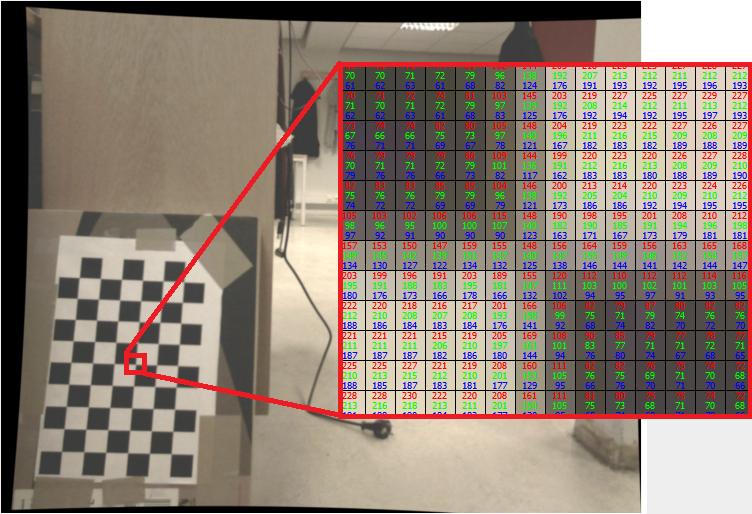
\includegraphics[scale=0.7]{SjakkMat}
\caption{Elements in a cv::Mat representing an image. This is a 3-channel image with 8 bit RGB colors.}
\label{fig:matGrid}
\end{figure}

\section{A Brief Introduction to Vision Based Autonomous Navigation}

\subsection{Simultanious Localization and Mapping (SLAM)}

Consider a robot that is placed in an unknown environment with no a priori information of the surroundings. If this robot is capable of solving the \gls{slam} problem, it is implied that it can build a map of the surroundings while it determines, simultaniously, where it is located on the same map. This section will, in brief, present some variants of and solutions to the \gls{slam} problem. From \cite{SLAMp1} a preliminary description of the \gls{slam} problem is based on the following parameters at time $k$ is:
\vspace{-10pt} % Remove exessive whitespace
\begin{description}
	\item[\boldmath$x_k$:] "State vection describing position and orientation of the vehicle"\cite{SLAMp1}.
	\item[\boldmath$u_k$:] Control input at time $k - 1$. Used to drive the vehicle to $x_k$. 
	\item[\boldmath$m_i$:] The position of the $ith$ landmark. The true position is assumed to be time invariant.
	\item[\boldmath$z_{ik}$:] Observed position of the $ith$ landmark relative to the vehicle at time $k$.
	\item[\boldmath$X_{0:k} = \{ x_0, x_1, ... , x_k\} = \{ X_{0:k-1}, x_l \}$] A set of all previous vehicle locations. 
	\item[\boldmath$X_{0:k} = \{ x_0, x_1, ... , x_k\} = \{ X_{0:k-1}, x_l \}$] All previous control inputs.
	\item[\boldmath$X_{0:k} = \{ x_0, x_1, ... , x_k\} = \{ X_{0:k-1}, x_l \}$] All previous landmark observations.
\end{description}

\paragraph{Probabilistic SLAM}
Probabilistic \gls{slam} computes the probability distrobution $P(x_k,m|Z_{0:k},U_{0_k},x_0)$ at all time steps $k$\cite{SLAMp1}, i.e. the joint probability that the robot is in state \boldmath$x_k$ and that the landmarks can be described by a map,\boldmath$m$, given historic inputs, landmark observations and vehicle states. The solution algorithm can be implemented in two steps: A time update based on the last updated observation history and current input, and a measurment update where $P(x_k,m|Z_{0:k},U_{0_k},x_0)$ is computed based on bayes theorem. 


\paragraph{EKF-SLAM}

The inclusion of \gls{awgn} leads to the application of the \gls{ekf} to the \gls{slam} problem\cite{SLAMp1}.
\paragraph{MonoSLAM}

MonoSLAM by Davison et. al. (2007) is the first successful vision based real-time \gls{slam} algorithm\cite{monoSLAM}. The algorithm works by maintaining a probabilistic 3d map of a sparse set of landmarks. The map is continously updated by an \gls{ekf}. Landmarks are chosen based on som prominent features in the surroundings. In the algorithm, they are represented as flat surfaces with a certain orientation in 3d space. This solution will approximate the fact that the appearence of a feature will change based on the position from where they are observed.

\paragraph{The Kinect Sensor and SLAM}

The Kinect sensor has been a remarkable contribution to the field of \gls{slam} and computer vision. It is a cheap sensor capable of generating high quality, but noisy, depth maps at $30 Hz$. By applying \gls{slam} to the real-time depth data, it is possible to generate a very accurate 3d reconstruction of the surroundings.


\section{The Pinhole Camera Model}

\subsection{Model Description}

\begin{wrapfigure}{r}{0.65\textwidth}
	\vspace{-10pt} % Remove exessive whitespace
	\centering
	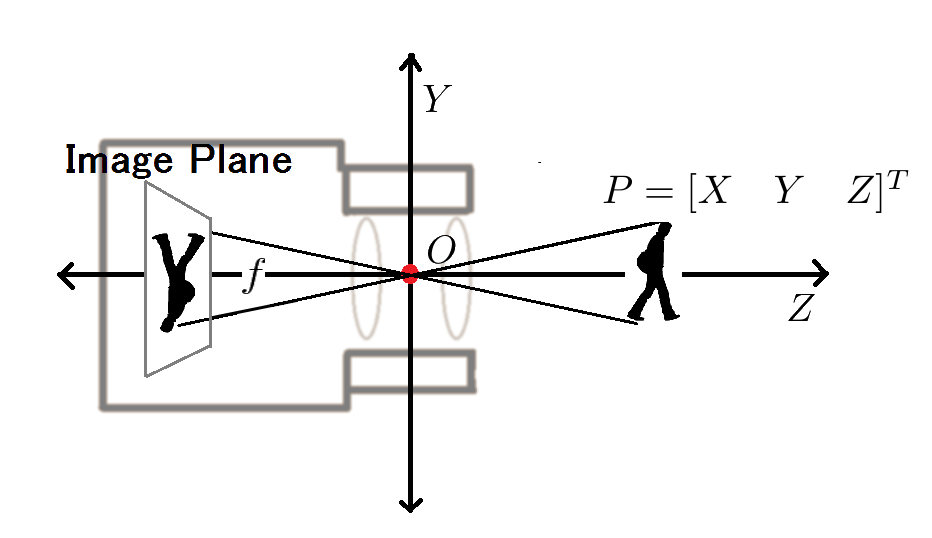
\includegraphics[width=0.7\textwidth]{pinhole}
	\caption{\label{fig:pinhole}Geometry of a pinhole camera.}
	\vspace{-10pt} % Remove exessive whitespace
	\label{phantompic}
\end{wrapfigure}

Figure \ref{fig:pinhole} illustrates the geometry of a pinhole camera. In a pinhole camera, light reflected from some object in a scene will be projected onto an image plane inside the camera house. The light is projected through the "pinhole", that is the camera projection point $O$, which is located at the origin. Imagine that a single ray enters the camera house through the pinhole, before it hits and exites a sensor element on the image plane. The values retreived from these sensor elements will make up the pixels in an image. The focal length $f$ is the distance from the projection point $O$ to the image plane $\pi$. In a true pinhole camera the image plane will be located behind the lens and the projection point $O$, and the scene projection will be rotated by $180^{\circ}$. A virtual image plane placed in front of $O$ is intended to make the figure more straightforward and the mathmatics easier. 

\begin{equation}
M = \begin{bmatrix}
f_x & 0 & c_x \\
0 & f_y & c_y \\
0 & 0 & 1
\end{bmatrix}
\label{eq:pinhole}
\end{equation}

"Learning OpenCV" by Gary Bradski\cite{oreillycv} shows how a pinhole camera can be modelled by a 3 by 3 camera matrix $M$ (equation \ref{eq:pinhole}). This model accounts for two important differences between the ideal and real pinhole camera. First, the imaging chip will often be displaced from the optical center. This displacement is described by the parameters $c_x$ and $c_y$. The second real world problem is that the pixels on the image sensor are shaped as rectangles, not squares. This is accounted for by $f_x$ and $f_y$, the focal lengths in the $x$ and $y$ direction given in pixels. These values are the product of the actual focal length $f$ and size of the individual imager elements $s_x$ and $s_y$. The reason for using these values in the camera model is because $s$ and $f$ cannot be measured without actually dismantling the camera\cite{oreillycv}.

\subsection{Camera Distortion}

A downside of the otherwise cheap and useful pinhole camera is camera distortion. The distortion is usually severe enough to render the camera useless as a sensor if it is not calibrated. Calibration in OpenCV accounts for radial and tangential distortion by finding five distortion coefficients \cite{3dCalib}:

%\vspace{-1em}
\begin{equation}
Distortion_{coefficients} = (k_1 \quad k_2 \quad p_1 \quad p_2 \quad k_3)
\label{eq:distortion}
\end{equation}
%\vspace{-0.2em}
\textbf{where} 
%\vspace{-1.1em}
\begin{equation*}
p_i \quad with \quad i \in \left\{1, 2\right\}
\end{equation*}
%\vspace{-0.3em}
\textbf{are the radial distortion constants, and}
%\vspace{-0.2em}
\begin{equation*}
k_i \quad \textrm{with} \quad i \in \left\{1, 2, 3\right\}  
\end{equation*}
%\vspace{-0.5em}
\textbf{are the tangential distortion constants.} 
%\vspace{-0.5em}

\section{Perspectives and Vanishing Points}

\begin{wrapfigure}{r}{0.5\textwidth}
	\vspace{-10pt} % Remove exessive whitespace
	\centering
	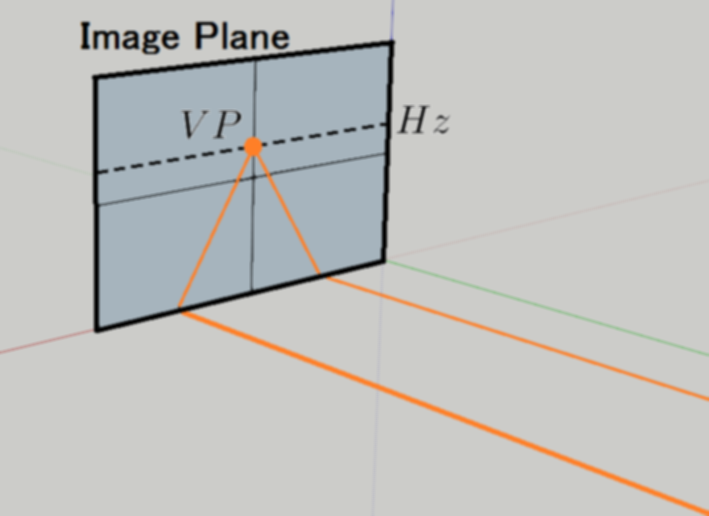
\includegraphics[width=0.5\textwidth]{VpConseptBl}
	\caption{\label{fig:VpConseptBl}Two parallel lines are projected onto an image plane, where they form two lines. These projected lines converge towards a vanishing point on the horizon.}
	\vspace{15pt} % Remove exessive whitespace
\end{wrapfigure}

\paragraph{Vanishing Points}

A vanishing point is the result of prespective projection. A prespective can be described as the way a 3d world appears when it is projected on a two-dimentional surface. Consider a set of two parallel lines in 3d space that are projected onto an image plane. If these two lines are not parallel to the image plane, their projected representatons will converge to a vanishing point. If the lines are parallel to the image plane, their corresponding vanishing points will be at infinity. The projected lines are formed by the projection lines, that is the direct lines from the parallel lines and the projection center $O$ (figure \ref{fig:pinhole} and \ref{fig:StereoSpace}). Figure \ref{fig:VpConseptBl} illustrates the consept of vanishing points with two parallel horizontal lines.

\paragraph{Perspective Transformations}

When the intrinsic camera parameters (equation \eqref{eq:pinhole}) and distortion coefficients (equation \ref{eq:distortion}) have been calculated, it will be possible to map a point in the outside 3d world to the image plane. This knowlegde allows perspective transformations. A perspective transformation can be used to transform a wall viewed at an angle to an observation point that is perpendicular to the wall. Likewise, the view of a road from a car can be transformed to a birds-eye representation. This birds-eye view can for example be used in combination with a \gls{lidar}\cite{oreillycv}.

\section{Stereo Vision and Depth Perception}

Stereo vision and depth perception is one of the core topics within this report. Here, the theory behind a method using two cameras is presented, while some additional methods are mentioned to provide context. 

\subsection{Various Methods}

Methods for depth perception in computer vision can be separated into two main categories, active and passive\cite{autorobot}. Active sensors will usually project a light pattern onto the scene to be perceived, before sensing how this pattern is displaced by the topology of the scene. The Kinect sensor and 3d-scanners using laser light are typical examples of active sensors. Passive depth perception makes use of many of the same cues we use to perceive depth. The most common passive sensors extract the depth information by observing observing a scene from at least two different positions. 

Optical flow is another important method for depth perception. Optical flow may be either active or passive. The passive variant requires  only one camera, but depends on motion and a stream of images to extract depth information.\cite{optflwdepth} \cite{optflwego} Observing how much some chosen features in a scene has moved in the image frame at $t = 1$ compared to the frame at $t = 0$ is the basis of depth sensing from optical flow. When the camera moves through a scene where all objects are stationary, objects that are far away will naturally have an optical flow field with a smaller magnitude than objects that are close. 

\subsection{Stereoscopic Vision in General}

In this project, passive stereoscopic vision is achieved by using two identical (in theory) cameras placed on the same plane. The gist of passive stereoscopic vision is based on the fact that objects close to the camera pair will have a large displacement from the left to the right camera compared to objects that are further away. This concept is illustrated in figure \ref{fig:3dScene}.

\begin{figure}
\centering
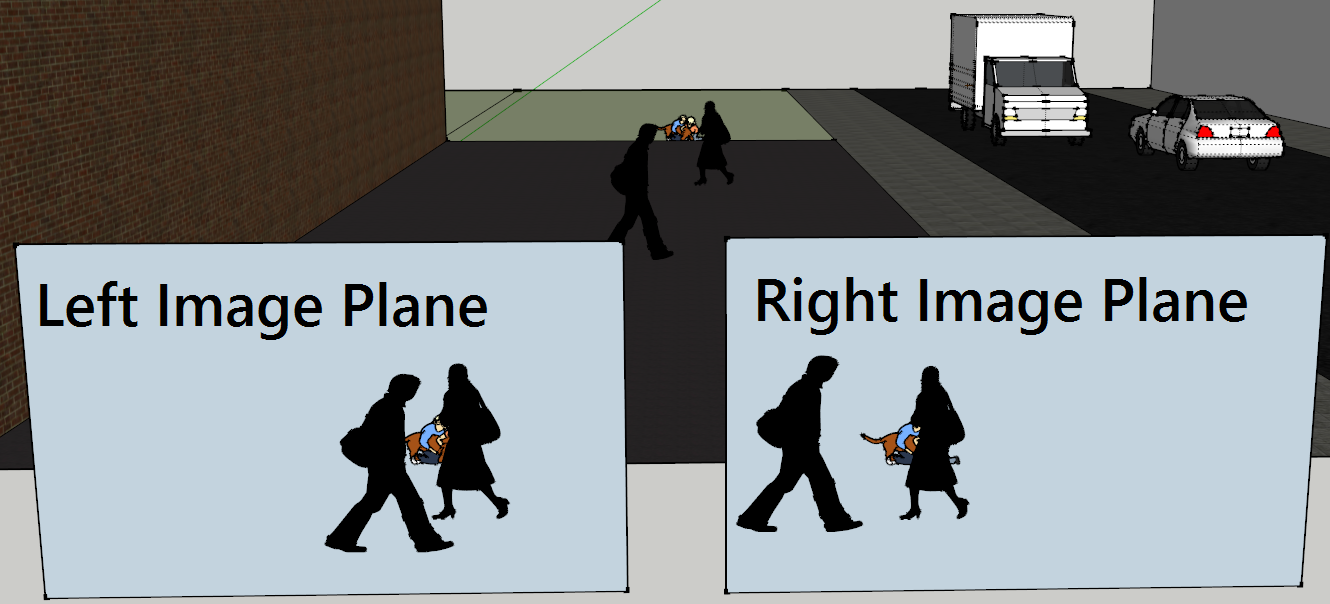
\includegraphics[scale=0.4]{3dScene}
\caption{\label{fig:3dScene}Left to right displacement on the image plane based on distance.}
\end{figure} 

\paragraph{Stereo Cameras}

Figure \ref{fig:StereoSpace} shows an ideal stereo camera model.  The model comprise two pinhole camera models where the virtual image planes are located on the same plane. The two image planes are separated by a horizontal translation $B$ which is called the baseline. This implies that the projection point $O_L$  in the left camera, relates to the projection point $O_R$ on the right camera through $B$: $O_R = O_L + B$. Each of the two image planes has a left handed pixel based coordinate system $u,v$, i.e. the origin is in the top left corner and the opposite pixel is in the bottom right corner. 

\begin{figure}
\centering
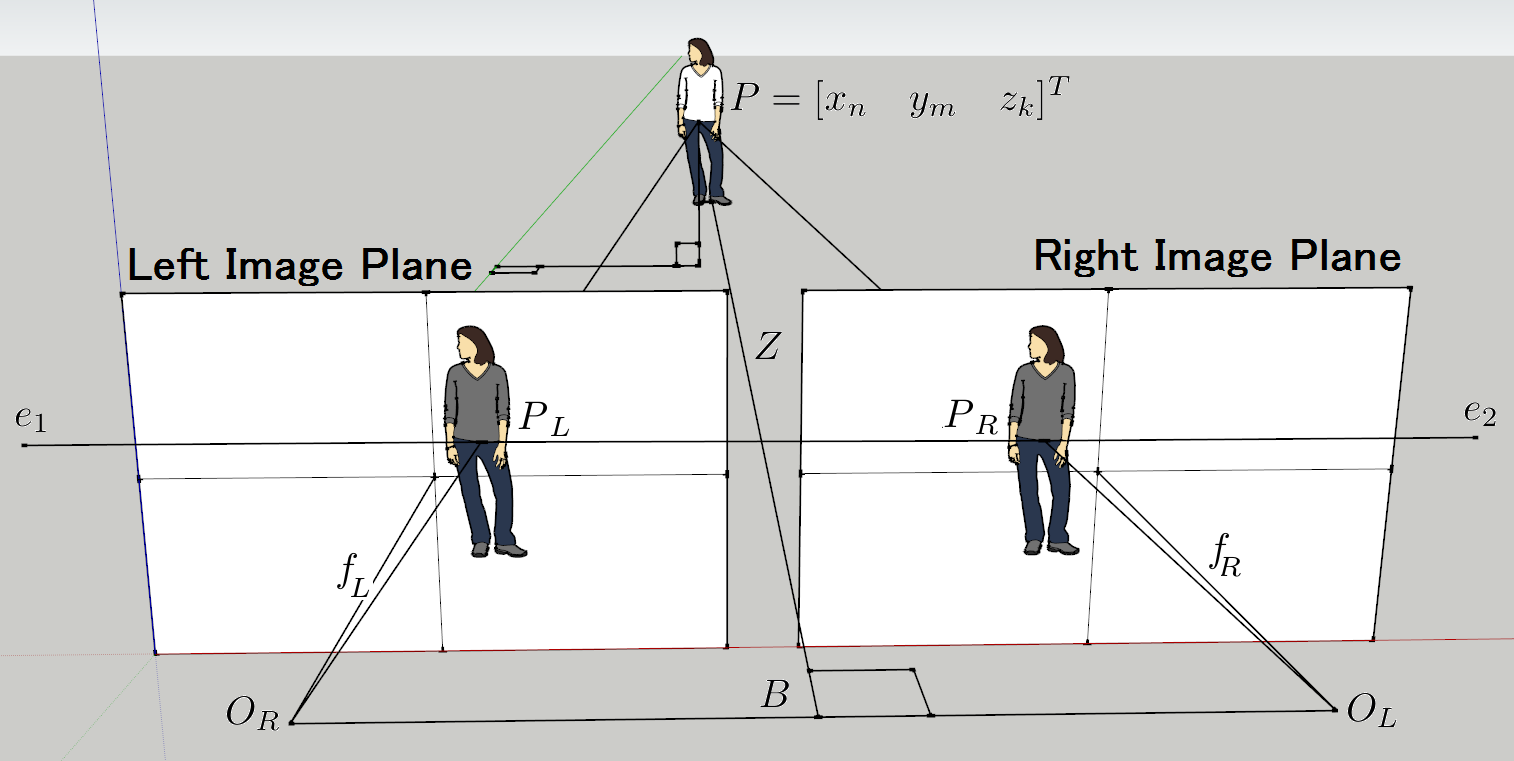
\includegraphics[width=1\textwidth]{StereoSpace}
\caption{\label{fig:StereoSpace}Geometry of rectified stereo vision.}
\end{figure}

\begin{wrapfigure}{r}{0.5\textwidth}
	\vspace{-10pt} % Remove exessive whitespace
	\centering
	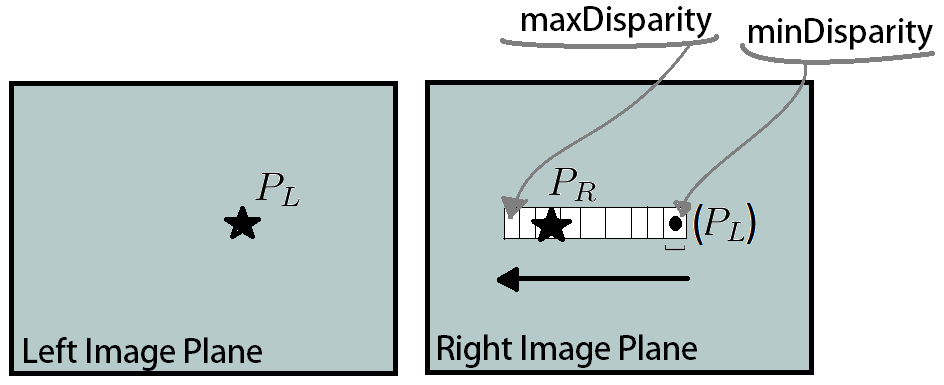
\includegraphics[width=0.6\textwidth]{blockMatching}
	\caption{Geometry of rectified stereo vision.}
	\label{fig:blockMatching}
\end{wrapfigure}

\subsection{Stereoscopic Vision in OpenCV}

The prebuilt version of OpenCV 3.0.0 comes with two stereo matching algorithms: \gls{bm} Block Matching (StereoBM) and Semi Global Block Matching (StereoSGBM)\cite{hirschmullerstereo}. Additional algorithms are available if OpenCV is built with, e.g. CUDA. Both algoritms require a rectified pair of images as input. The basic idea of block matching is illustrated in figure \ref{fig:blockMatching}. The algorithm will search for blocks in the right image that corresponds to similar blocks in the right image. In \cite{hirschmullerstereo}, this process is described as "pixelwise matching of mutual information". This search for mutual information is simplified significantly if the search direction can be limited to a one dimentional constraint: a horizontal line. This is easy to do, given that the assumption of coplanar image planes holds. The disparity is a measure of how far the matching blocks are displaced from each other. 
